\documentclass{article}
\usepackage{handover}
\usepackage{float}


\begin{document}
\doctitle{Monitoring}{Music Podcast Player}
\section{Introduction}
Another facet of our project is the Logging, located in the backend, and our Metrics Dashboard, which lives in an AWS Cloudwatch Instance. Our logs cover virtually every interaction a user may have with the application, including both errors, action, and response logging. Our logs are primarily focused on tracking user movements and error tracking.
\section{Logging Coverage}
\begin{itemize}
    \item \textbf{200} -- Any successful response from the server returned to the user
    \item \textbf{400} -- Malformed JSON in Request \& Arguments Did Not Match Expected Scheme
    \item \textbf{404} -- The Requested Resource Could Not Be Found
    \item \textbf{409} -- The Field Is Already in Use
    \item \textbf{429} -- The Server is Receiving Too Many Requests to Process the Current One
    \item \textbf{502} -- The Internal API Response was Invalid \& The External API Response was Invalid
    \item \textbf{503} -- The External API Used for this response was invalid
    \item \textbf{504} -- We Were Unable to Reach the Internal API \& We Were Unable to Reach the External API 
\end{itemize}
\section{Cloudwatch}
\begin{figure}[H]
    \centering
    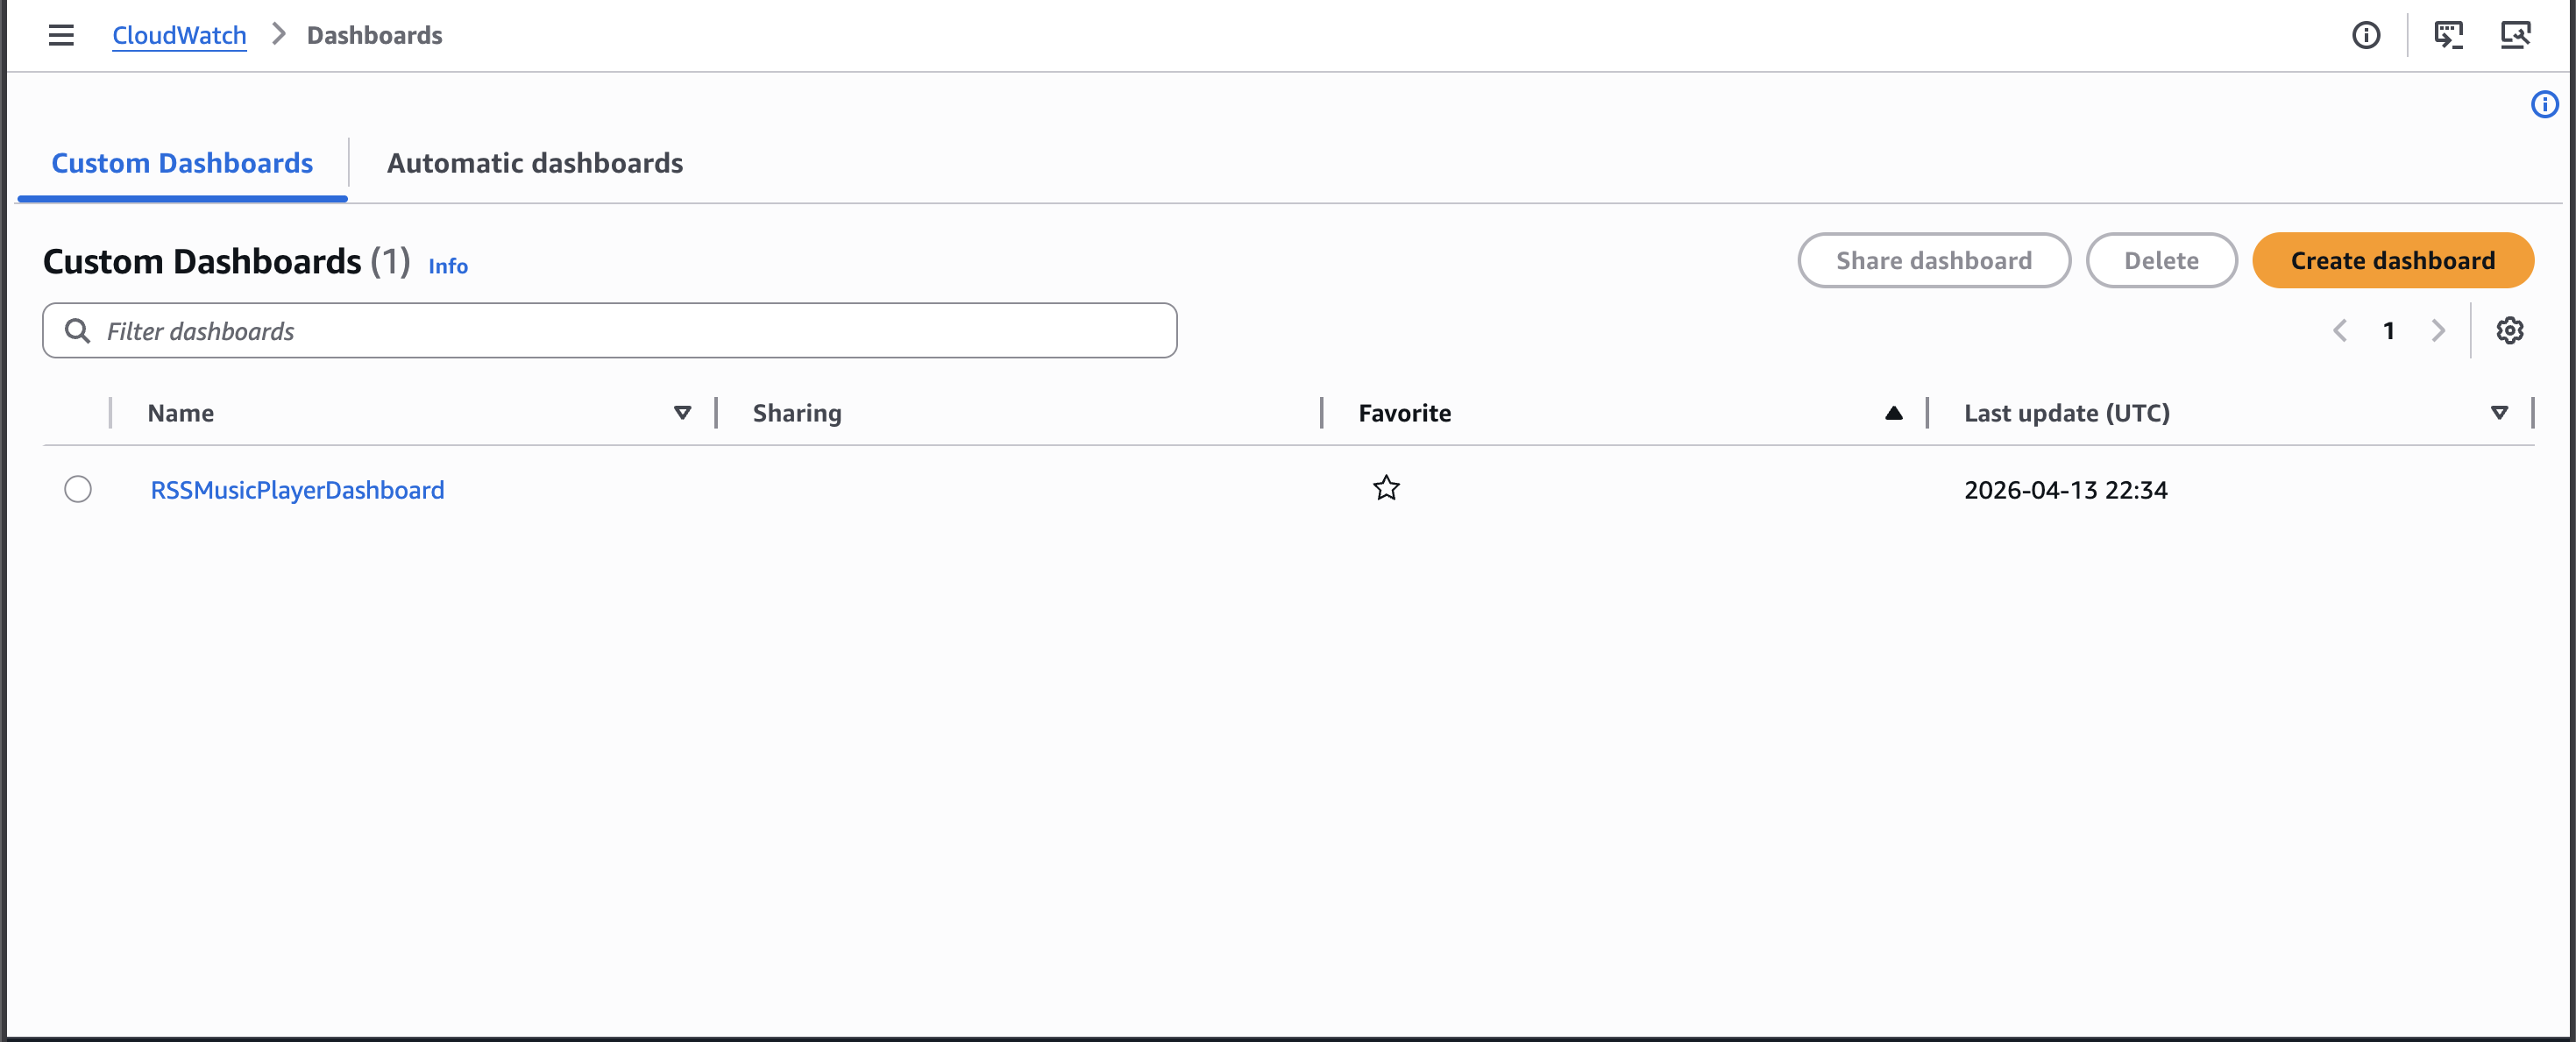
\includegraphics[width=0.5\linewidth]{cw-dashboard.png}
    \caption{Dashboard Creation}
    \label{fig:placeholder}
\end{figure}
After connecting to the CDK and navigating to cloudwatch, you'll likely be faced with this screen. TheRSSMusicPlayer Dashboard is the initial base dashboard that  displays the metrics for all current logs in the application. There are also non-custom dashboards that display pre-configured metrics for the application as well, but are not configurable. Cloudwatch runs alongside the EC2 Instance and waits for the agent to send the logs to cloudwatch. 
\section{Creating New Logs}
To create new logs, you must go into the cdk snapshot of the backend, and find the errors.py file. Inside this file there is a class of enums that relate to the errors. To include a request or response error, you update the class with expected error, then create the enumerated type for it.
\begin{figure}[H]
    \centering
    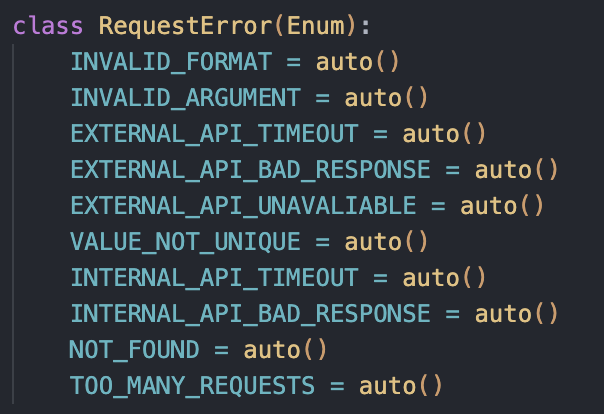
\includegraphics[width=0.4\linewidth]{error-class.png}
    \caption{Error Class}
    \label{fig:placeholder}
\end{figure}
Creating new logs, after updating the class, is as simple as following the structure outlined in the logging config. Each log should contain an error, message, and code to complete it. After the enumerated type is created, it should be added to the class, to be included in the logs that will be returned. 
\begin{figure}[H]
    \centering
    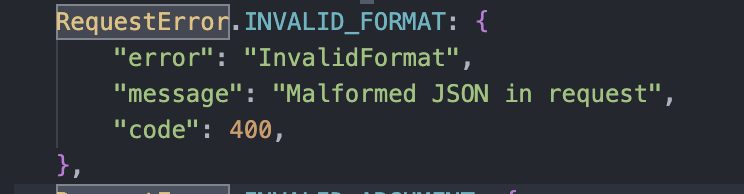
\includegraphics[width=0.5\linewidth]{request.png}
    \caption{Error Format}
    \label{fig:placeholder}
\end{figure}
To update logging structure, navigate to the loggingconfig.py file and locate the log request function. Here, you can update the log structure and add different tags and types to extend them. In here, you can also update the order of keys for the logs. These should only be updated if you decide to change the entire structure of the logs as well. 
\begin{figure}[H]
    \centering
    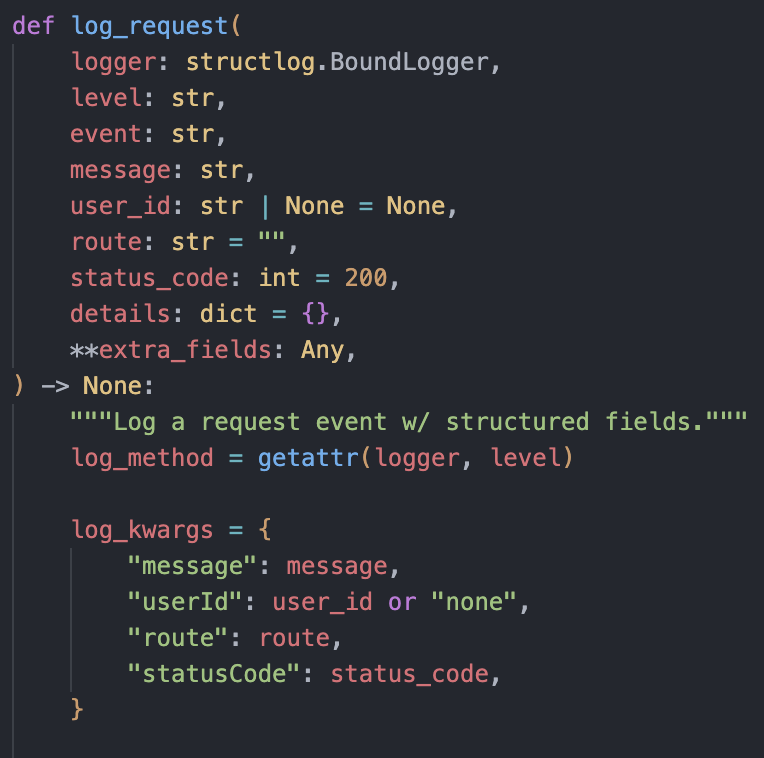
\includegraphics[width=0.4\linewidth]{log-structure.png}
    \caption{Log Structure}
    \label{fig:placeholder}
\end{figure}
\section{Creating New Metrics}
To create new metrics, you have to navigate to the CDK stack file and locate the functions that create the dashboards and metrics. These metrics are updated on a new deployment of the CDK, and a new metric or dashboard will only be able to be seen on the new deployment. To create a new metric, you have to add a new metric filter to the log group. To add the log to the metric, you have to add a filter pattern and metric value. The mertic value is how much your log increments when the filter pattern was detected.
\begin{figure}[H]
    \centering
    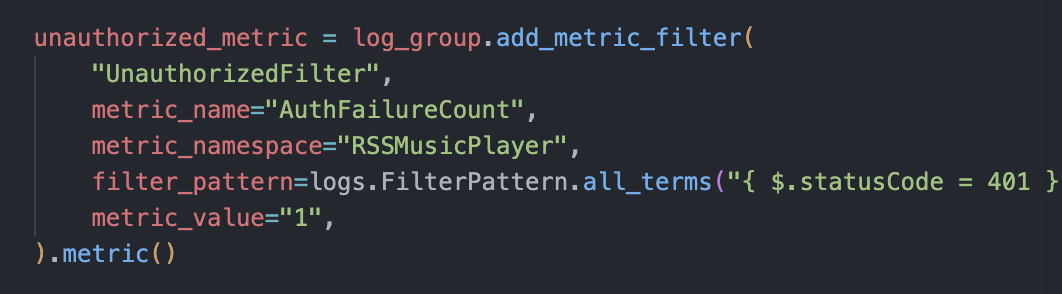
\includegraphics[width=0.5\linewidth]{metric.png}
    \caption{Metric Structure}
    \label{fig:placeholder}
\end{figure}
Right below, you will find how to create a new dashboard for the cloudwatch instance as well. To create a new dashboard you have to name and create an update interval for the dashboard. After this, you have reference the metrics you want to include in the dashboard. Once these a referenced and the new dashboard is deployed, you should be able to navigate to your AWS Console and view your newly created metrics and dashboard.
\begin{figure}[H]
    \centering
    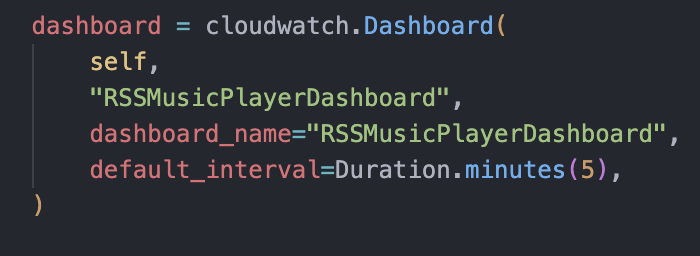
\includegraphics[width=0.5\linewidth]{dashboard.png}
    \caption{Dashboard Structure}
    \label{fig:placeholder}
\end{figure}
\end{document}